\documentclass[a4paper,12pt]{article}
\addtolength{\oddsidemargin}{-1.cm}
\addtolength{\textwidth}{2cm}
\addtolength{\topmargin}{-2cm}
\addtolength{\textheight}{3.5cm}
\newcommand{\HRule}{\rule{\linewidth}{0.5mm}}
\makeindex

\usepackage{longtable}
\usepackage[pdftex]{graphicx}
\usepackage{makeidx}
\usepackage{hyperref}
\usepackage{verbatim}
\hypersetup{
    colorlinks=true,
    linkcolor=blue,
    filecolor=magenta,      
    urlcolor=cyan,
}


% define the title
\author{IMAPKD}
\title{ Project Tender}
\begin{document}
\setlength{\parskip}{6pt}

% generates the title
\begin{titlepage}

\begin{center}
% Upper part of the page       

\includegraphics[width=1\textwidth]{./University_of_Pretoria_Logo.PNG}\\[0.4cm]    
\textsc{\Large Project Tender}\\[0.5cm]
% Title

{ \huge \textsc Project: VizARD(Augmented Reality Data Visualization) }\\[0.4cm]\
{ \huge \textsc Client: EPI-USE Labs  }\\[0.1cm]\

{ \huge \textsc Team: IMPAKD  }\\[0.1cm]\

\textsc{\Large Team Members}\\[0.3cm]

{\Large Diana {Obo}} \\[0.3cm]

{\Large Kudzai {Muranga}} \\[0.3cm]

{\Large Priscilla {Madigoe}}\\[0.3cm]

{\Large Sandile {Khumalo}}\\[0.5cm]

\textsc{ Department Of Computer Science, University of Pretoria}\\[0.3cm]
\textsc{Date: 2 May 2016}\\[0.3cm]

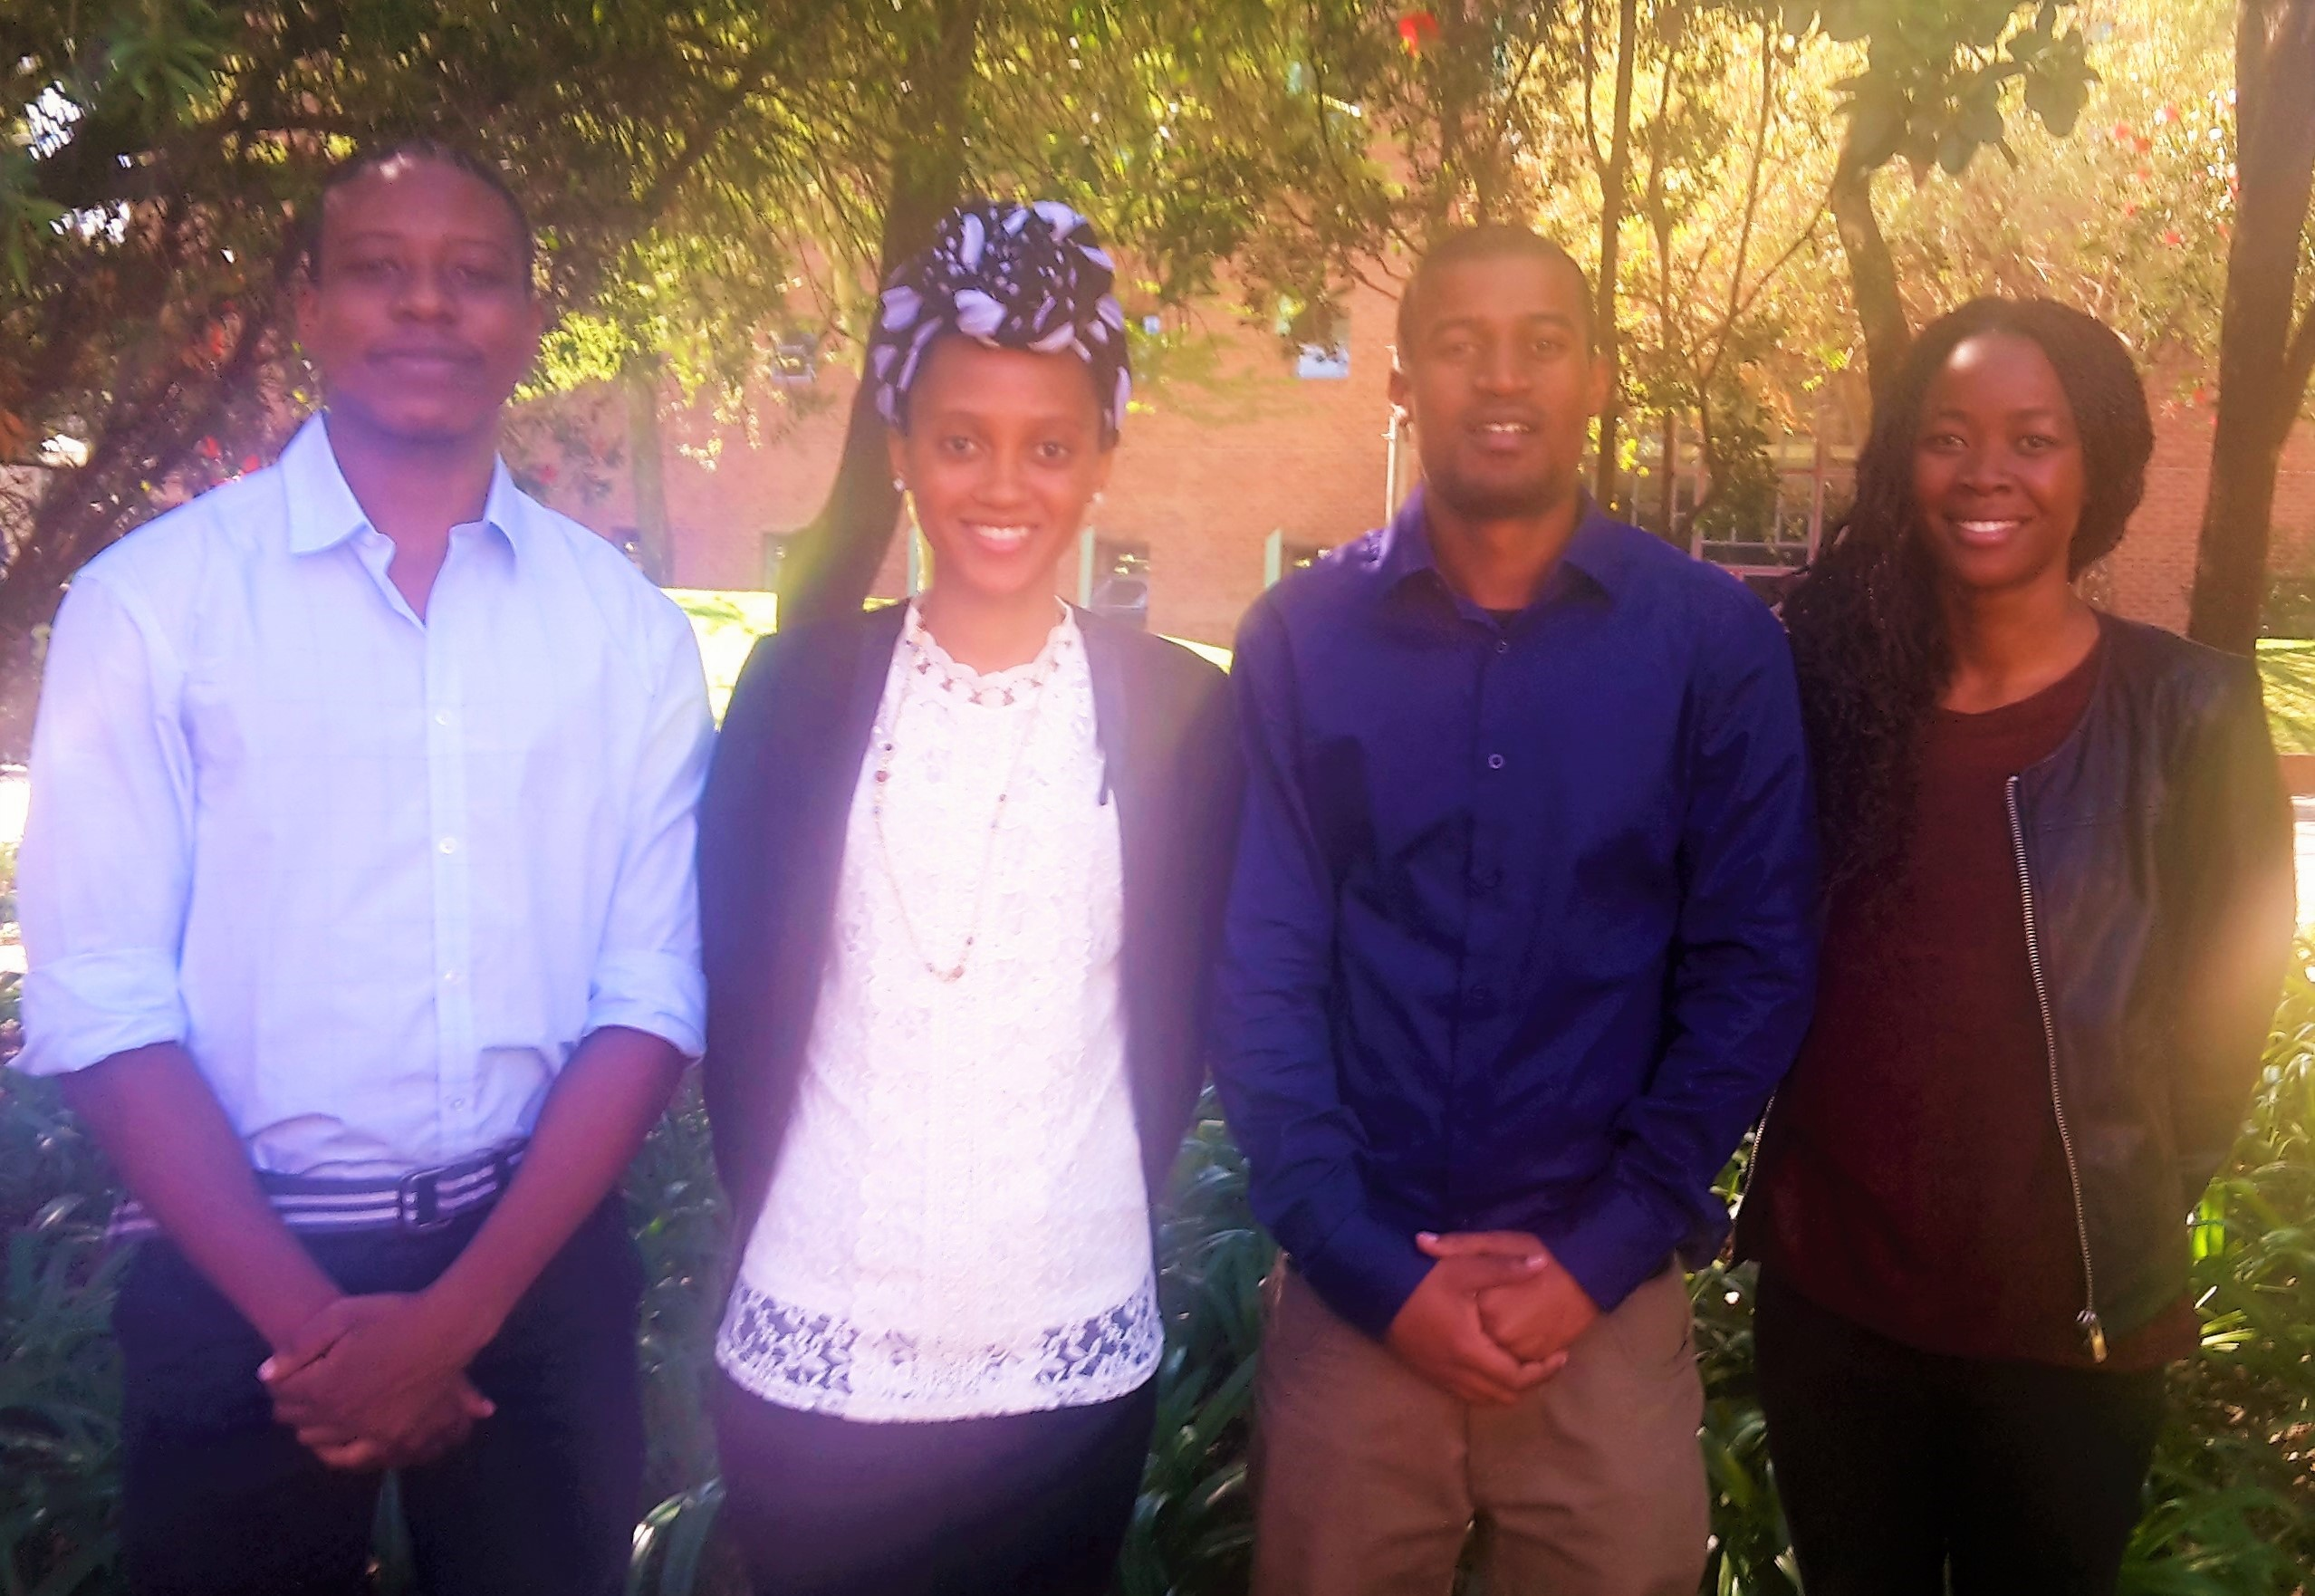
\includegraphics[width=4in]{./IMAPKD.jpg}

\vfill
% Bottom of the page
\end{center}
\end{titlepage}

\newpage
\section{Meet the Team Members}

%Priscilla Madigoe's Section - beginning

\begin{center}
{\Large Priscilla {Madigoe}} \\[0.3cm]
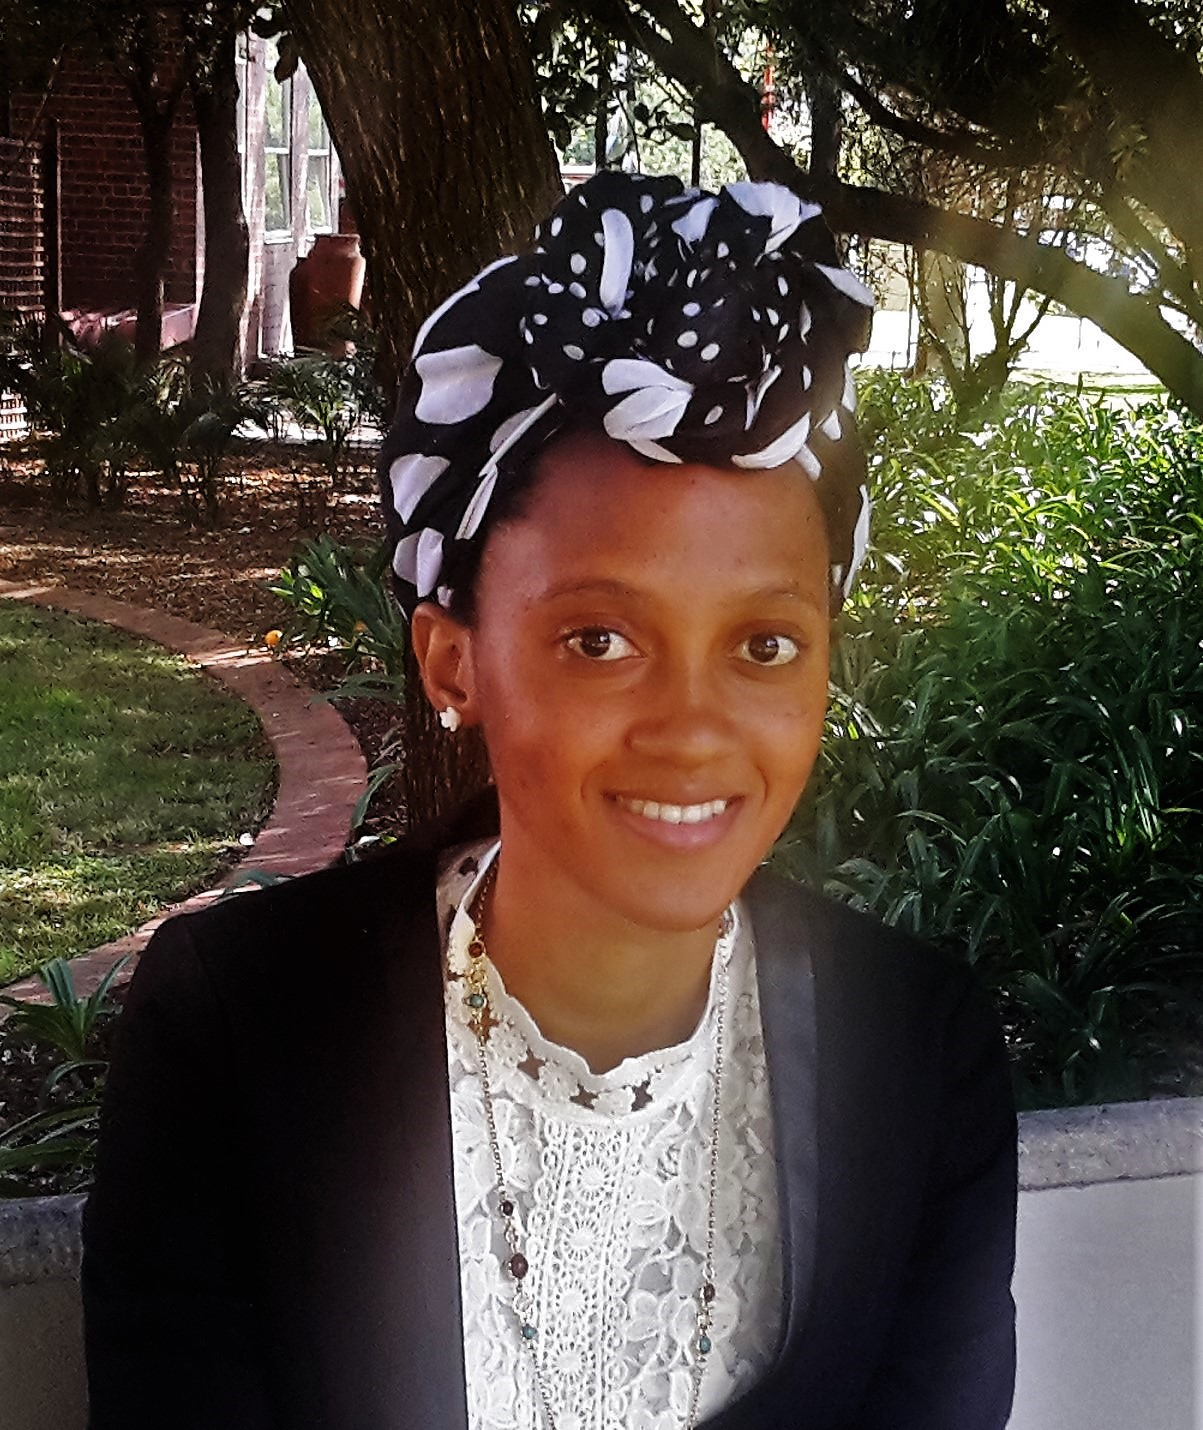
\includegraphics[width= 2in]{P.jpg}\\[0.4cm] 
\end{center}

\begin{itemize}
\item {\large \underline{\textbf{Interests}}}\\[0.2cm]
My interests include Computer Programming, Electronics, Computer Graphics, Robotics, travelling, photography, music, sports and reading novels.
\\
\item {\large \underline{\textbf{Technical Skills}}}

	\begin{itemize}
		\item Computer Programming with sound knowledge of Java, C/C++, MatLab, WebGL and Web-related 					programming languages.
		\item Complex Problem-Solving using scientific and mathematical principles.
		\item System Analysis to determine how a computer software should behave in set conditions.
		\item Quality Control Analysis to evaluate the performance and quality of computer software.
	\end{itemize}
\bigskip
\item {\large \underline{\textbf{Past Experience}}}\\[0.2cm]
The Software Engineering module had a preparatory project called the Mini Project that was created to give students a real-world experience of software development. I took part in the project and I have learnt the process of software development, team work and different technologies used to develop computer software. 
\\
\item {\large \underline{\textbf{Non-Technical Skills}}}\\[0.2cm]
My non-technical skills include critical thinking, reading comprehension, writing, effective listening, social perceptiveness and active learning. 
\\
\item {\large \underline{\textbf{Reason for Interest in the Project}}}\\[0.2cm]
I would like to expand my knowledge on Computer Graphics and Augmented Reality as I am currently enrolled in an elementary Computer Graphics course.

\end{itemize}
%Priscilla Madigoe's Section - end 

\newpage

% Diana Obo's Section - start
\begin{center}
{\Large Diana {Obo}} \\[0.3cm]
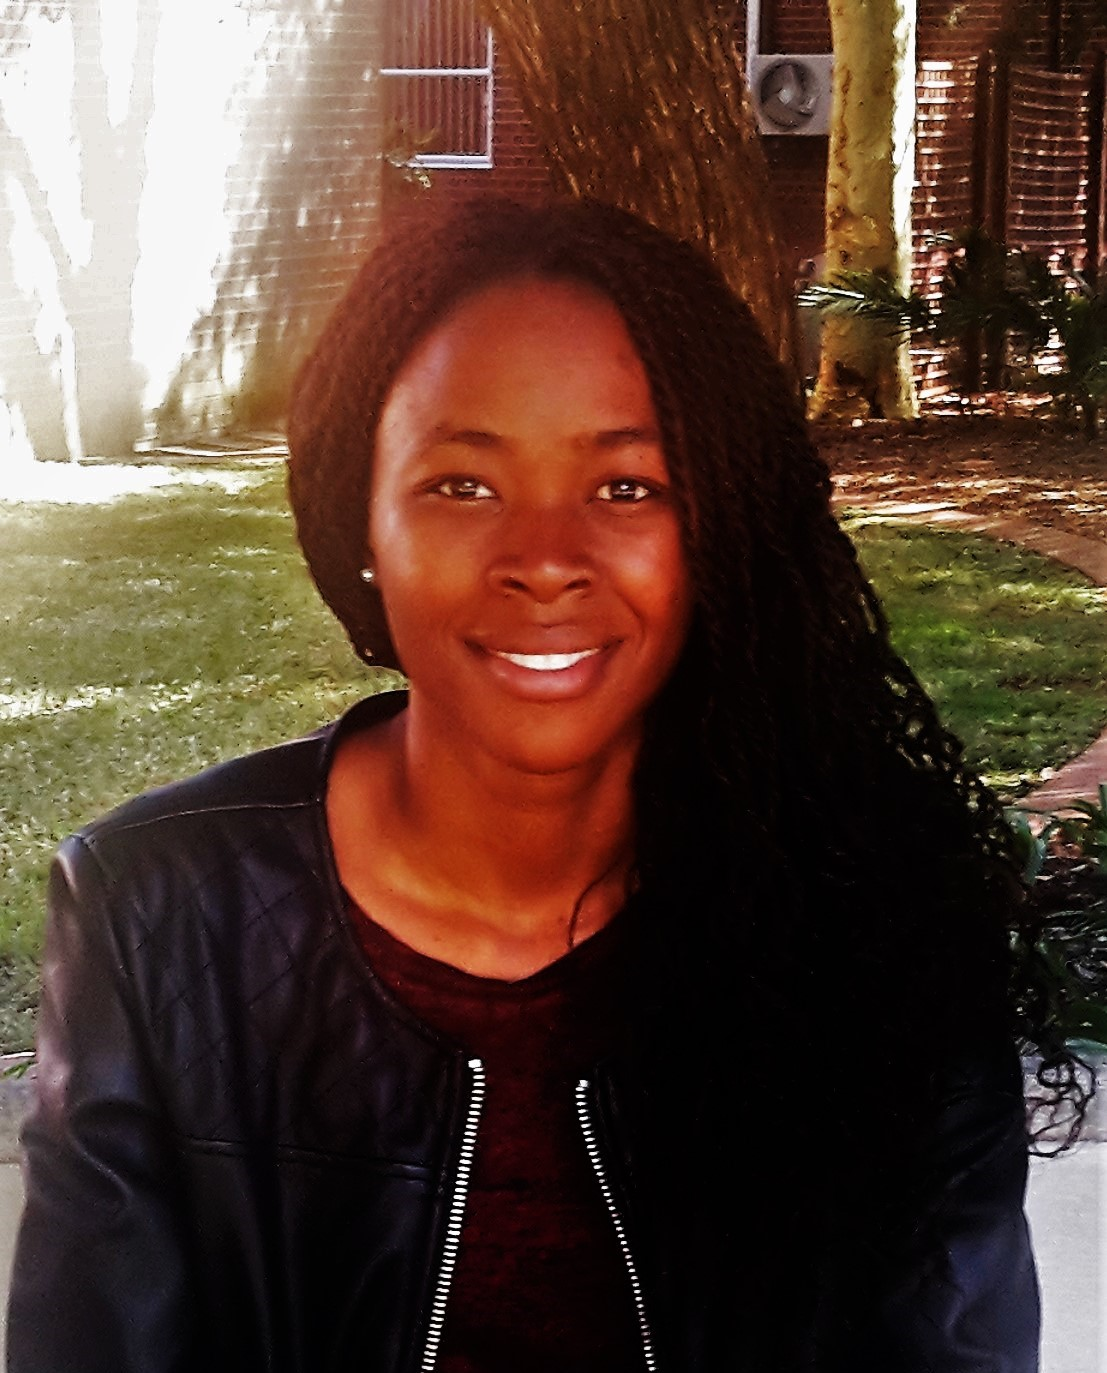
\includegraphics[width= 2in]{Diana.jpg}\\[0.4cm] 
\end{center}

\begin{itemize}
\item {\large \underline{\textbf{Interests}}}\\[0.2cm]
My interests are travelling, game development, web development and anime. I also enjoy learning about new technologies and watching a lot of discovery channels and documentaries.

\item {\large \underline{\textbf{Technical Skills}}}
	\begin{itemize}
		\item I have sound knowledge of Java, C++, HTML, CSS, Javascript, C\#, MatLab
		\item Mobile development (android studio) 
		\item 3DS MAX.
		\item Ember.js and  handlebar.js
	\end{itemize}
\bigskip
\item {\large \underline{\textbf{Past Experience}}}
\begin{itemize}
\item I participated in this year's Standard Bank IT Challenge.
\item I did an internship at a small company named Lepsta where I did web development.
\end{itemize}
\bigskip
\item {\large \underline{\textbf{Non-Technical Skills}}}
\begin{itemize}
\item Willingness to learn
\item Team player
\item Organised
\item Diligent
\item Reliable
\end{itemize}
\bigskip
\item {\large \underline{\textbf{Reason for Interest in the Project}}}\\[0.2cm]
Since I am Interested in Game development, anime and I’ve worked with 3DS max, this project will expand my knowledge in Augmented Reality and Computer Graphics.

\end{itemize}
%Diana Obo's Section - end

\newpage

% Kudzai Muranga's Section - start
\begin{center}
{\Large Kudzai {Muranga}} \\[0.3cm]
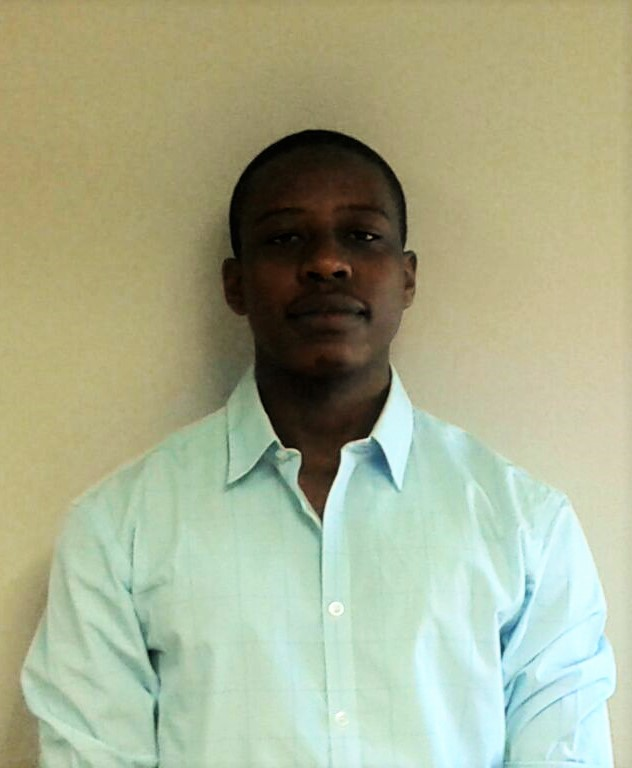
\includegraphics[width= 2in]{Kudzai.jpg}\\[0.4cm] 
\end{center}

\begin{itemize}
\item {\large \underline{\textbf{Interests}}}\\[0.2cm]
I am an avid reader, I love fantasy novels the most. I like to keep myself up to date with the current affairs of the world. I am also interested in learning anything new that concerns science, technology and business.
\\
\item {\large \underline{\textbf{Technical Skills}}}
	\begin{itemize}
		\item I have sound knowledge of Java, C++, HTML, CSS, Javascript, C\# and mobile development 
		\item Artificial Intelligence experience.
		\item Business Management knowledge
		\item Project Management
	\end{itemize}
\bigskip
\item {\large \underline{\textbf{Past Experience}}}
\begin{itemize}
\item Participated in the Standard Bank IT Challenge.
\item Invited to the Hello Group Open Day where I participated in a coding challenge using Java.
\end{itemize}
\bigskip
\item {\large \underline{\textbf{Non-Technical Skills}}}
\begin{itemize}
\item I am interested and open to learning new things
\item Disciplined
\item Organised
\item Critical Thinking
\end{itemize}
\bigskip
\item {\large \underline{\textbf{Reason for Interest in the Project}}}\\[0.2cm]
I am interested in this project because I feel that it would allow me to use programming abilities extensively and teach me new and exciting skills.
% Kudzai Muranga's Section - end

\newpage
%Sandile Khumalo's Section - start
\end{itemize}
\begin{center}
{\Large Sandile {Khumalo}} \\[0.3cm]
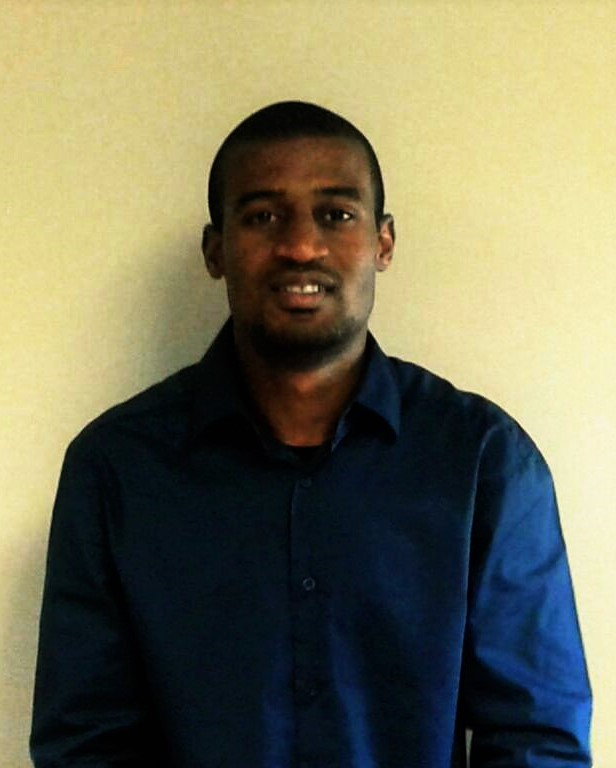
\includegraphics[width=2in]{Sandile.jpg}\\[0.4cm] 
\end{center}



\begin{itemize}
\item {\large \underline{\textbf{Interests}}}\\[0.2cm]
My interest are coding , reading on new exciting, technologies ,watching and reading about football. I also enjoy weightlifting.


\item {\large \underline{\textbf{Technical Skills}}}

	\begin{itemize}
		\item I am comfortable and have experience coding in these languages; c++, java, c\#, php, html, javaScript, bash. I also have done 64 bit assembler language and I have experience in MINIX.
	\end{itemize}
\bigskip
\item {\large \underline{\textbf{Past Experience}}}\\[0.2cm]
I have done a project in my software development class that is similar, it incorporates  most of the technologies and frameworks used in the work place when developing big projects.
\\
\item {\large \underline{\textbf{Non-Technical Skills}}}\\[0.2cm]
 I am a hard working student, I am dedicated, I believe if there is a will, the is a way.Especially as a developer because most of the solutions are there, someone has done it before.It's a matter of good research and good understanding of the task at hand. I am willing to learn from every experience. 
\\
\item {\large \underline{\textbf{Reason for Interest in the Project}}}\\[0.2cm]
I find this project challenging and exciting, There is a lot to learn from it.It would be great to work on the augmented reality feature and expand my knowledge.

\end{itemize}

%Sandile Khumalo's Section - end
\newpage
\section{Project Execution}
\end{document}

